\chapter{Background}
\sectionreference{If you are familiar with medical imaging and MRI feel free to skip to section \ref{background:svr}. These first few sections are intended to give a brief introduction to the field.}

% ------------------------- %
% ---- MEDICAL IMAGING ---- %
% ------------------------- %
\section{Medical Imaging}\label{background:medicalimaging}
The field of medical imaging came into existence with the discovery of x-rays in 1895 by Wilhelm R\"{o}ntgen\cite{rontgen}. This meant that for the first time it was possible to peek into the human anatomy without having to physically open it up. This revolution came at a cost however as at the time the dangers of high doses of radiation were not understood and many of the pioneers died as a result of exposure\cite{xraydeath}.

Radiology, the use of ionizing radiation to image objects, was greatly refined over the years; contrast agents were developed which made fields like angiography (imaging of blood vessels) possible\cite{infinityhistory} and the doses used were refined to dramatically decrease the associated risks. X-rays have been used successfully in medical imaging ever since and in the 70s the invention of the CT (X-Ray Computed Tomography) scanner allowed them to be used to produce 3D images of the body.

It was not until the 1980s that magnetic resonance imaging (MRI) was first used for medical diagnosis. MRI is based on the principles of nuclear magnetic resonance (NMR), which had been used in chemical analysis since the 40s\cite{bshr:mallard}.

MRI can be used to create anatomical images by examining the varying water content in different parts of the body. More recently MRI has been used to create functional images of the brain by using the same principals to detect blood flow\cite{fmri}. Unlike CT, which uses x-rays, MRI does not require the use of any ionizing radiation to perform the scan.

As with all medical imaging techniques the benefits and risks need to be weighed up before a scan is performed. When imaging fetuses the risks are higher than normal and so in general CT scans tend not to be used wherever possible. MRI however, like US (ultrasound), is not associated with known adverse fetal effects\cite{pregnancyimagingguidelines}.

% ------------------------- %
% ---------- MRI ---------- %
% ------------------------- %
\newpage
\section{MRI}\label{background:mri}
MRI uses a strong magnetic field and radio waves to produce images of the body. MRI can be used to produce 2D, 3D and even 4D images and has the advantage that it doesn’t use any ionizing radiation during the scanning process\cite{howmriworks}.

MRI is able to detect the amount of water that is contained in different types of tissue in the body by exploiting a property of protons called spin. Water is detected because the nuclei of each hydrogen atom in water consists of a single proton.

MRI applies a strong uniform magnetic field to the area being imaged which causes the spins of the protons to line up with the direction of the field. Some of the protons line up in the same direction, with low energy, and some line up opposing the magnetic field, which have high energy.

When a particular radio frequency is then applied some of the lower energy protons flip to become higher energy and oppose the magnetic field, when the radio waves are stopped these protons then flip back, emitting a radio wave that can be detected. The resonant frequency of radio wave that is required to excite the protons depends on the strength of the magnetic field. This property allows an area to be scanned by applying a gradient magnetic field and varying the radio frequency.

Different weightings of scan exist: T1-weighted scans are best for visualizing fat, calcification, hemorrhage, thyroid, liver and bone marrow whereas T2-weighted scans accentuate water content. Different sequences can also be acquired: SSFSE (Single Shot Fast Spin Echo) works by acquiring each slice of the image in sequence whereas 2DGRE (Gradient Echo) acquires all of the slices simultaneously.

If the contrast that can be achieved with MRI is insufficient for the imaging then a contrast agent, such as gadolinium, can be administered to enhance it.

\section{Fetal MRI}\label{background:fetalmri}

Since MRI, like US, is a non-invasive procedure that doesn’t use ionizing radiation it is ideal for use in fetal imaging\cite{fetalmri}. While US remains the most common imaging modality used during pregnancy MRI has a number of advantages; in particular better contrast in soft tissue allows organs to be better differentiated. However, US remains more widely available, easier to apply, easier to staff and cheaper and so is unlikely to be replaced as the main fetal imaging tool in the near future.

There are no known side effects associated with using MRI, however it is currently recommended to wait until the 17th or 18th WG (week of gestation) before performing MRI. This is partly a precautionary measure but also before then the size of the fetus and amount of movement limits the usefulness of the scan\cite{fetalmri}.

% -------------------------- %
% ---- Super-Resolution ---- %
% -------------------------- %
\newpage
\section{Slice-to-Volume Reconstruction}\label{background:svr}
The main challenge with using MRI for fetal imaging is dealing with movement. One of the ways that this effect can be minimized is to reduce the time spent acquiring the image, which is typically achieved by using a large slice thickness. A typical slice thickness used when scanning a fetal brain is 3mm; considering that the size of the brain may only be 50mm this resolution limits the diagnostic potential.

SVR (Slice-to-Volume Reconstruction) is a technique that solves these problems by taking in a number of these motion corrupted stacks, aligns them and then builds a high resolution reconstruction. Individual slices are assumed to have been acquired fast enough that the movement within then is negligible, however the target may move in between slices as each stack takes a few minutes to acquire.

Figure \ref{fig:svroverview} outlines the SVR procedure.

\begin{figure}[H]
    \centering
	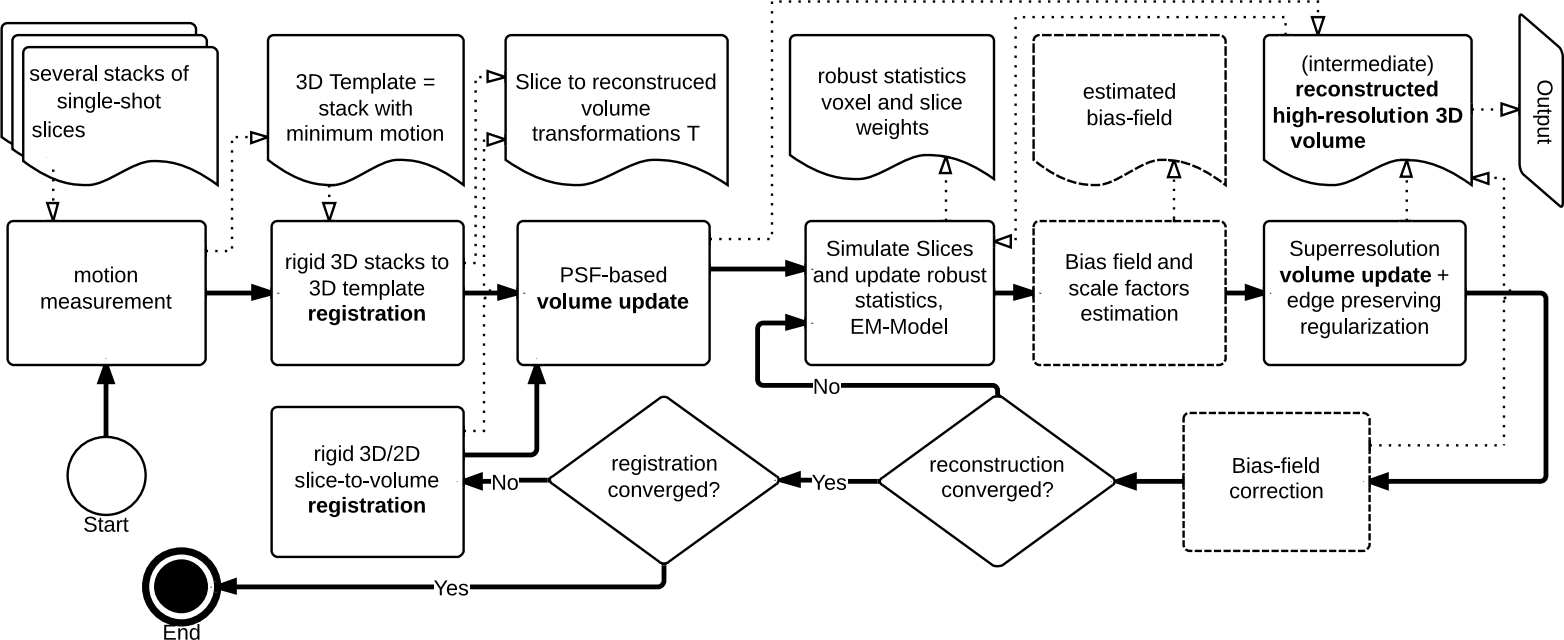
\includegraphics[width=1.0\textwidth]{images/background/svr_overview.png}
    \caption{SVR Overview. Adapted from \cite{gpureconstruction}}
    \label{fig:svroverview}
\end{figure}

The first step is to find the stack with the least movement; this is then used as a target to register all the other slices to. Continuous point spread functions (PSFs) are used to model the intensity of each input stack at continuous points in space. This essentially allows an initial reconstruction to be performed by sampling the PSFs of each of the input stacks.

An outlier detection phase is then performed; this involves the inverse of the transform used to align every slice to the volume being used to determine what the slice should have looked like, based on the reconstruction. These simulated slices can then be compared to the originals and applying EM (Expectation Maximization), an iterative procedure, determines how likely each point is to be an outlier.

A noise removal and edge preserving step is then implemented before a super-resolution image of the current best reconstruction is produced, based on the probabilities that each point is an outlier. As the diagram illustrates this process is iterated until the registration process converges.

This process of combining many lower resolution stacks to create one high resolution image is known as super-resolution. With super-resolution the images must be taken such that the translation between them is known to sub-pixel accuracy. Having images where the pixels are interleaved in this way allows a higher resolution image to be constructed using interpolation. See figure \ref{fig:superresolution}.

\begin{figure}[H]
    \centering
	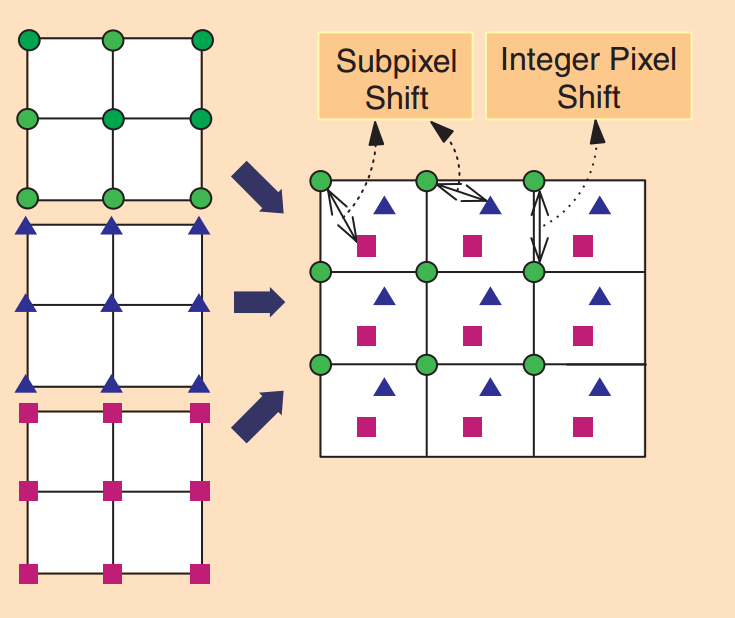
\includegraphics[width=0.8\textwidth]{images/background/super_resolution.png}
    \caption{Low resolution images aligned to sub-pixel accuracy. Adapted from \cite{superresolution2}}
    \label{fig:superresolution}
\end{figure}

\subsection*{Super-Resolution Overview}
The simplest form of super-resolution follows three steps:

\begin{enumerate}
	\item Registration
	\item Interpolation
	\item Post-processing
\end{enumerate}

The registration step is where the transformation between each image is established. Crucially this must be known to sub-pixel accuracy and must not be a whole number of pixels. If, for example, we had two images and one was taken exactly 1 pixels width to the right of the other then we see that both images will contain the same information, in effect we can generate one using the other. However, if the second image is known to be taken half a pixel's width to the right then there is the potential to extract more information.

Once we have registered our images we then interpolate points at a higher resolution, using a combination of the pixel values from each image at each point. There are a number of different interpolation algorithms that we can use; for example nearest neighbour or linear interpolation.

We can then perform post-processing on the final image to reduce the noise or blur. For example to reduce noise a Wiener filter can be used\cite{wienerfilter}.

% ------------------------- %
% ------- SVD / PCA ------- %
% ------------------------- %
\newpage
\section{SVD \& PCA}\label{background:svdpca}
The task of finding the next best scan plane given an uncertainty volume is a task that essentially involves fitting a scan plane to a set of uncertain points. SVD (Singular Value Decomposition) is one technique that has been successfully applied to solving this problem\cite{uncertaintysvd}.

SVD  breaks down a matrix, $A$, into three components: $U$, $D$ and $V$.

\begin{align}
& A = UDV* \nonumber \\
& \text{where} \nonumber \\
& A \text{ - the original matrix. (M x N)} \nonumber \\
& U \text{ - a unitary matrix. (M x M)} \nonumber \\
& D \text{ - a diagonal matrix containing the singular values. (M x N)} \nonumber \\
& V* \text{ - the conjugate transpose of V, a unitary matrix. (N x N)} \nonumber
\end{align}

Note that 'Unitary Matrix' means that $UU* = I$ or alternately $U^{-1} = U^T$. This is true where the matrix contains unit vectors.

Note that the 'Conjugate Transpose' ($*$) of a matrix is just the transpose of the matrix and additionally the complex conjugate of each entry is taken. If the matrix contains no complex values $U* = U^T$.

SVD comes in useful when performing PCA (Principal Component Analysis). PCA is used to take a dataset in $n$ dimensions and map it in such a way that you can describe it in less than $n$, whilst minimizing the information lost.

PCA takes as input a data matrix, X, which is a two dimensional table where each row represents an 'experiment' or 'data point' and each column is a property. Using the covariance of this data, i.e. how much each property varies in relation to every other property, the number of dimensions can be reduced.

To find the principal component we would like find the vector that maximizes the variance in the covariance matrix. This is found by extracting the eigenvalues of the covariance matrix.

\begin{align*}
& X \text{ - data matrix (demeaned)} \\
& XX^{T} \text{ - covariance matrix} \\
& \\
& \text{Since the covariance matrix is symmetric it can be diagonalized.} \\
& \\
& XX^{T} = WDW^{-1} \\
& \\
& W \text{ - eigenvectors of the covariance matrix} \\
& D \text{ - eigenvalues of the covariance matrix}
\end{align*}

Applying PCA to $X$ (and using the SVD substitution):

\begin{align*}
X &= UDV^T \\
& \\
XX^T &= (UDV^T)(UDV^T)^T \\
	&= (UDV^T)(VD^TU^T) \\
	&= UDD^TU \\
	&= UD^{2}U \\
	& \text{therefore} \\
UD^{2}U &= WDW
\end{align*}

We see that the eigenvalues are just the square root of the diagonal we get from SVD and the eigenvectors are the same. These eigenvectors form our new dimensions and we can reduce our data to $m < n$ dimensions by picking the $m$ with the largest eigenvalues.

% ------------------------ %
% -------- RANSAC -------- %
% ------------------------ %
\newpage
\section{RANSAC}\label{background:ransac}
RANSAC (Random Sample Consensus) is a technique for estimating model parameters given some sample data. Similarly to SVD it can be used for suggesting the next best scan plane.

Consider the task of trying to fit a line to some data which contains both correct points (inliers) and noisy data (outliers). The problem with simply minimizing the sum of squared errors to all of the points is that the outliers will distort the result such that the inliers are not perfectly described by the data. See figure \ref{fig:ransac}.

\begin{figure}[H]
    \centering
	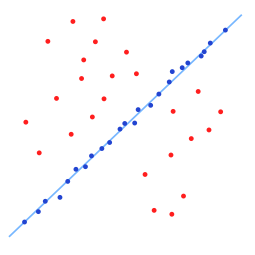
\includegraphics[width=0.4\textwidth]{images/background/ransac.png}
    \caption{Inliers are shown in blue, outliers shown in red. From \cite{ransac:image}}
    \label{fig:ransac}
\end{figure}

RANSAC gets over this problem using random sampling and iteration. It relies on there being more inliers than there are outliers so that statistically inliers will be chosen more frequently. The algorithm is composed of two steps which are repeatedly applied.

As many points are taken randomly from the data set as are needed to fully specify the model (e.g. you need two points to specify a line).

The points are then fit to the model and then all of the data points are compared to this model. If they differ by more than a threshold value they are discarded. If they fit the model they are put into this iterations ‘inlier set’.

A number of iterations are then performed and the winning iteration is the one with the largest inlier set. The final model is then either the model which gave the largest inlier set or alternatively the model can be generated using every point in the inlier set. This algorithm relies on certain parameters being tweaked to perform well:

\begin{itemize}
	\item threshold (how picky to be when discarding points)
	\item iterations (how many times to run the algorithm)
\end{itemize}

% -------------------------- %
% ---- Volume Rendering ---- %
% -------------------------- %
\newpage
\section{Direct Volume Rendering}\label{background:volumerendering}
MRI is a tomographic imaging technique which means that a 3D image is acquired in slices. The resulting scan is created by combining these slices to build a 3D volume. An MRI scan is often displayed in 2D by taking each slice and displaying it, however it is also possible to take all of the slices and view the scan in 3D. One technique for doing this is direct volume rendering.

Direct volume rendering is a technique for visualizing 3D volumetric data which does not generate any intermediate representation. The process uses ray tracing whereby rays are fired through each pixel in the image and properties of light, such as colour and opacity, are modelled to render the data \cite{nvidia:volumerendering}.

One ray is sent into the volume per pixel in the resulting visualization and samples are taken at regular intervals. Each sample point may not exactly hit a voxel in the volume and so the value will be interpolated from the neighbouring points. Linear interpolation can be used but may introduce some visual artefacts in which case more complex interpolation (such as piecewise cubic polynomials) can be used.

Each of these samples, which are just intensity values, need to be mapped to something that we can visualize. A transfer function is used to map intensity values to a colour and transparency. This transfer function can then be changed to highlight different features of our volume, for example we could make all values below a certain threshold completely transparent.

All of the samples along the ray are then combined to calculate the value of the pixel.

\begin{align*}
	C &= \sum\limits_{i=1}^n C_{i}\prod\limits_{j=1}^{i-1}(1 - O_j) \\
	O &= 1 - \prod\limits_{j=1}^n(1 - O_j) \\
	& \text{where} \\
	C_i &= \text{ colour at sample i} \\
	O_j &= \text{ opacity at sample j} \\
	C &= \text{ final colour} \\
	O &= \text{ final opacity}
\end{align*}

Note that if $O$ is greater than 0 then the colour is normalized (divided by $1 - O$).

% ---------------------------- %
% ---- Surface Extraction ---- %
% ---------------------------- %
\newpage
\section{Surface Extraction}\label{background:surfaceextraction}
Surface extraction is another technique that can be used to visualize volumetric data. Instead of visualizing the data directly, as in direct volume rendering, the volume is processed to build a geometric representation which can then be rendered.

This advantage of using surface extraction is that it is much cheaper to render\cite{surfacevsvolumerendering}. There is an initial penalty where the volume data is processed to extract surfaces but once this has been completed the rendering of geometric primitives is something that can be done rapidly by graphics hardware.

A common surface extraction algorithm is marching cubes. This algorithm works by examining the intensities of neighbouring voxels to tell whether or not the surface passes between them by comparing the values to a threshold value. 

The process is easier to visualize in 2D (marching squares), see Figure~\ref{fig:marching_squares}, but it can be simply extended to 3D.

\begin{wrapfigure}[16]{r}{0.6\textwidth}
  \vspace{-20pt}
  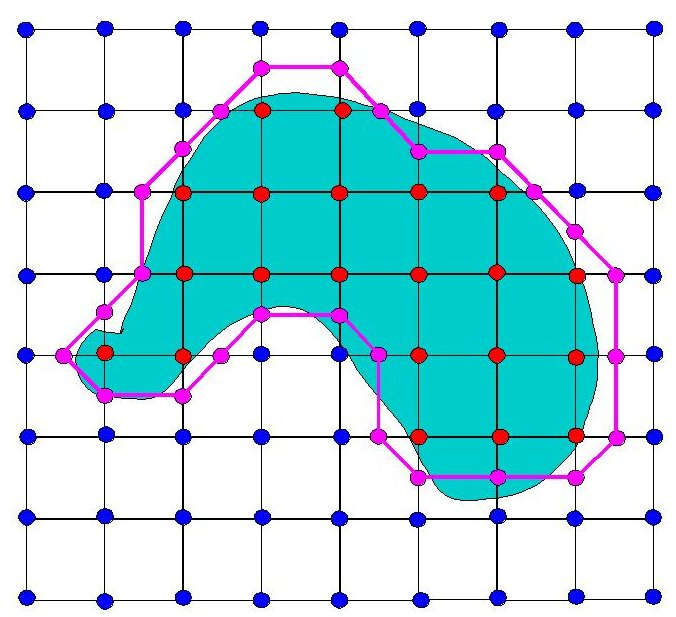
\includegraphics[width=0.6\textwidth]{images/background/marching_squares.jpg}
  \caption{Marching squares. From \cite{marching_squares:image}}\label{fig:marching_squares}
\end{wrapfigure}

The marching cubes algorithm generates as a result a mesh of triangles which can be reduced to the desired resolution by applying some mesh decimation techniques.

There are some constraints associated with using surface extraction for volume visualization. Firstly the number of primitives required to represent certain volumes may be prohibitively high. As an extreme imagine trying to extract surfaces from the volumetric representation of a dust cloud; in this case due to the shear quantity of particles it would not be practical to do so and in other situations an accuracy/efficiency trade off must be found.

There is also a certain amount of information loss with this technique: importantly individual intensity values are lost.

% ----------------------------------- %
% ---- Uncertainty Visualization ---- %
% ----------------------------------- %
\newpage
\section{Uncertainty Visualization}\label{background:uncertaintyvisualization}
Generally speaking uncertainty visualization tackles the problem of trying to represent the ambiguity or uncertainty in a data set or model. Most data visualization techniques implicitly assume that all of the data being used is perfect and because of this create visualizations that misleadingly represents values with greater precision than the underlying data is known to\cite{uncertaintyoverview}.

One of the reasons that a lot of visualizations neglect this is because it can be quite a difficult task. When creating a visualization there is an inherent restriction on the number of dimensions that you can exploit to represent information.

Consider the general problem of creating a visualization from an n-dimensional dataset in 3D. In this case we need to find a mapping from each dimension in our data to a 'dimension' in our visualization. The dimensions we can control are space (x, y, z), colour (RGB/HSV) and time. The art of data visualization is to find an intuitive mapping to these and to creatively reuse these dimensions to illustrate different features.

The issue when it comes to uncertainty visualization is that most of these dimensions have already been used up with the data itself and so finding intuitive representations for uncertainty is difficult.

To get an idea of what is possible with visualization techniques here are some examples that have been applied successfully in the past.

\begin{figure}[H]
    \centering
	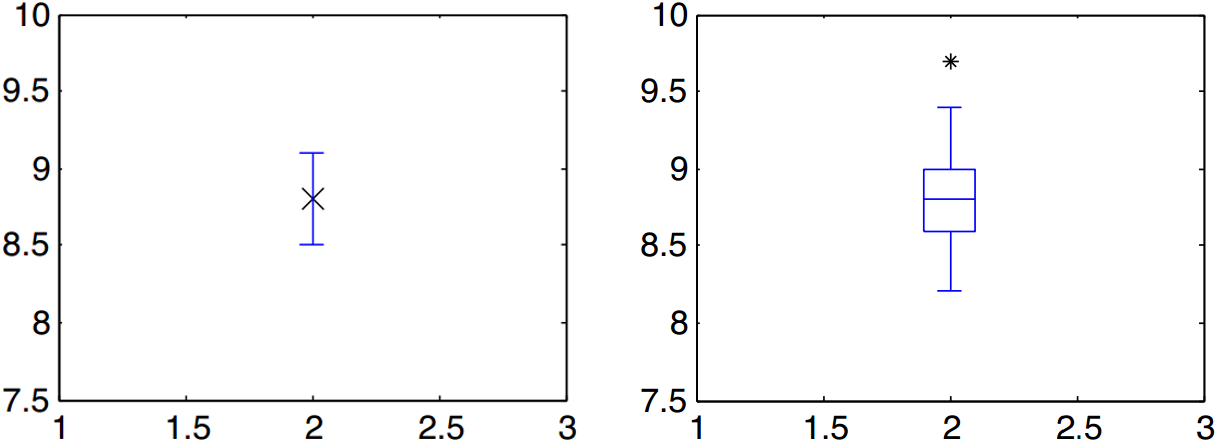
\includegraphics[width=0.8\textwidth]{images/background/error_bars.png}
    \caption{Left: Error Bar, Right: Box and Whisker Plot. From \cite{uncertaintyoverview}}
    \label{fig:error_bars}
\end{figure}

Error bars are possibly the simplest form of uncertainty visualization possible and are commonly found on graphs. They make use of one spatial dimension. An extension of this technique is the box and whisker plot which adds some idea of variance and range. An example of both is shown in Figure~\ref{fig:error_bars}.

\begin{figure}[H]
    \centering
	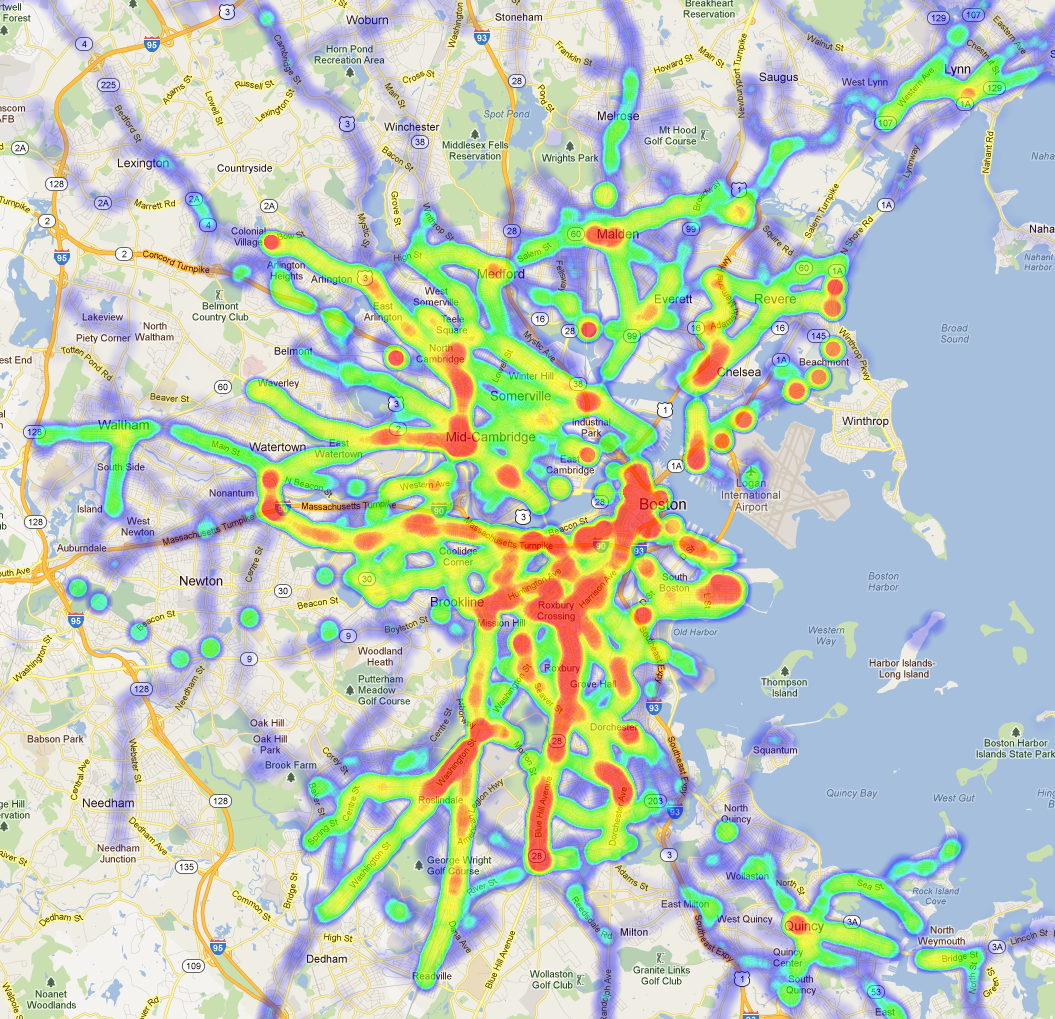
\includegraphics[width=0.4\textwidth]{images/background/heatmap.png}
    \caption{An example heatmap. From \cite{heatmap}}
    \label{fig:heatmap}
\end{figure}

Colour can be very effective at communicating information. A heatmap uses a range of colours to represent intensity data in a certain range. Transparency can also be used though care must be taken to not over complicate the visualization. An example of using both colour and transparency is shown in Figure~\ref{fig:heatmap}.

Time is a useful dimension to exploit but is more suited to some visualizations than others. When combined with a different dimension, such as colour, an animation can be produced that can draw the viewers attention.

In particular a team at the Vienna University of Technology have written a paper on 'attractive flicker' which is designed to draw the viewers attention to a particular point in a cluttered scene\cite{attractiveflicker}. Figure~\ref{fig:flicker} illustrates this idea.

\begin{figure}[H]
    \centering
	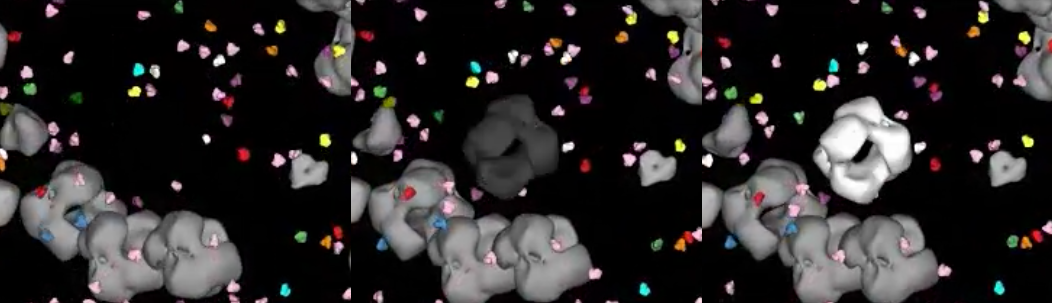
\includegraphics[width=0.8\textwidth]{images/background/flicker.png}
    \caption{Three frames show a molecule being highlighted as it flickers. From \cite{attractiveflicker}}
    \label{fig:flicker}
\end{figure}

When visualizing uncertainty the extreme to draw attention to should be considered. A lot of uncertainty visualizations focus on high uncertainty areas, for example brighter colours on a heatmap or larger error bars, but it may be the case that the viewer is interested in areas of low uncertainty as this is what they can draw conclusions from.